% ============================================================================
% TP2 -- Manual y procedimiento funcional de la SDR (entregable OE2)
% Plantilla basada en el TP1 (RE-TP-001). Un solo archivo .tex. Necesita en la
% misma carpeta: logo_fiuba.png, logo_materia.png y fig_ventana_demo.png.
% Compilar con pdfLaTeX (Overleaf: Menu > Compiler > pdfLaTeX).
% ============================================================================
\documentclass[11pt,a4paper]{article}

\usepackage[utf8]{inputenc}
\usepackage[T1]{fontenc}
\usepackage[default]{sourcesanspro}
\usepackage[spanish,es-tabla,es-nodecimaldot]{babel}
\usepackage[a4paper,margin=2.5cm,headheight=14pt]{geometry}
\usepackage{graphicx}
\usepackage{float}       % permite la opcion [H] en figuras y tablas
\usepackage{booktabs}
\usepackage{array}
\usepackage{longtable}
\usepackage{enumitem}
\usepackage{amsmath}
\usepackage{xcolor}
\usepackage{fancyhdr}
\usepackage{tikz}
\usetikzlibrary{babel,positioning}   % babel evita el choque entre TikZ y los atajos < > del español
\usepackage[hidelinks]{hyperref}

% ---------------------------------------------------------------- datos ----
\newcommand{\codigo}{OE2}
\newcommand{\version}{1.1 (borrador)}
\newcommand{\fecha}{26 de octubre de 2026}

% Columna de tabla con texto alineado a la izquierda
\newcolumntype{L}[1]{>{\raggedright\arraybackslash}p{#1}}

\pagestyle{fancy}
\fancyhf{}
\lhead{\small \codigo{} -- Manual y procedimiento funcional de la SDR}
\rhead{\small Versión \version}
\cfoot{\small \thepage}

\setlist{itemsep=1pt,topsep=3pt}
\setlength{\emergencystretch}{3em}   % deja cortar los renglones con nombres de archivo largos

\begin{document}

% ============================================================== caratula ====
\begin{titlepage}
  \centering
  \vspace*{0.5cm}
  % logo de la facultad a la izquierda y logo de la materia a la derecha
  \begin{minipage}[c]{0.56\textwidth}
    \centering
    
\includegraphics[width=\textwidth]{logo_fiuba.png}
  \end{minipage}\hfill
  \begin{minipage}[c]{0.34\textwidth}
    \centering
    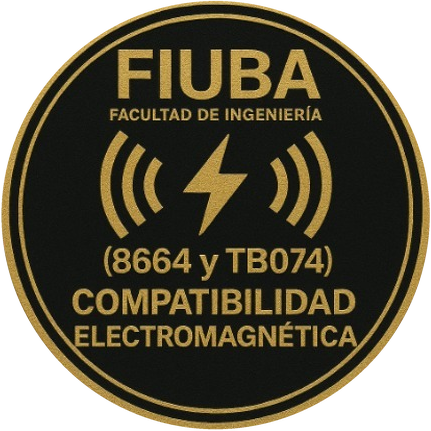
\includegraphics[width=\textwidth]{logo_materia.png}
  \end{minipage}\par
  \vspace{0.8cm}
  {\large Universidad de Buenos Aires -- Facultad de Ingeniería\par}
  {\large Compatibilidad Electromagnética (8664 y TB074)\par}
  {\large Trabajo Práctico N.\textsuperscript{o}~2 -- Entregable OE2\par}
  \vspace{1.6cm}
  {\LARGE \bfseries Manual y procedimiento funcional de la SDR\par}
  \vspace{0.6cm}
  {\Large Comb Generator basado en Software Defined Radio (SDR)\par}
  \vspace{0.8cm}
  {\large Código: \textbf{\codigo} \qquad Versión: \textbf{\version}\par}
  \vfill
  \begin{tabular}{ll}
    \toprule
    Autor               & Martín Ledesma \\
    Docentes            & Pablo Marino Belcaguy \\
                        & Walter Gustavo Fano \\
    Fecha               & \fecha \\
    \bottomrule
  \end{tabular}
  \vspace{1cm}
\end{titlepage}

% ====================================================== control de cambios ==
\section*{Control de versiones}
\begin{tabular}{@{}llp{8cm}@{}}
  \toprule
  Versión & Fecha & Cambios \\
  \midrule
  0.1 (borrador) & 21 de octubre de 2026 & Plantilla. \\
  1.0 (borrador) & 26 de octubre de 2026 & Primera versión completa, con el flujo del EXP-28. \\
  1.1 (borrador) & \fecha & Versión corta. \\
  \bottomrule
\end{tabular}

\tableofcontents

% ============================================================================
\section{Introducción}

\begin{itemize}
  \item Manual de uso de un generador peine hecho con una SDR bladeRF 2.0 micro xA9 y GNU Radio. Sirve para verificar la cadena de medición de emisiones radiadas (RE) de un laboratorio de EMC y seguir su continuidad en el tiempo.
  \item Pensado para cualquier laboratorio, cámara o facultad que tenga una SDR similar, un analizador portátil y un receptor de EMC.
  \item Alcance: 96 líneas de 50~MHz a 1~GHz, una cada 10~MHz, calibración por cable, calibración irradiada contra CISPR~11 grupo~1 clase~A a 3~m y patrón para repetir la emisión otro día. El ensayo en sí está en el RE-TP-001 (TP1).
  \item Flujo de referencia: EXP-28, en \texttt{SDR/A9\_22\_EXP28\_Peine\_calibracion\_CISPR} del repositorio del proyecto.
\end{itemize}

\begin{table}[H]
  \centering
  \small
  \begin{tabular}{@{}L{4.4cm}L{6.9cm}L{2.5cm}@{}}
    \toprule
    Requerimiento & Cómo lo cumple & Estado \\
    \midrule
    CW con frecuencia, amplitud y permanencia controladas & Línea fija, ganancia de TX, amplitud por línea y tiempo por línea & Cumplido hasta 1~GHz \\
    CW en 1,5 y 2~GHz & La xA9 llega a 6~GHz, el flujo a 1~GHz & Pendiente \\
    Barrido de 100~MHz a 1~GHz cada 50~MHz & Barrido de 50 a 1000~MHz cada 10~MHz & Cumplido \\
    Generador de varios tonos & Una línea por vez, juntadas con MAX HOLD & Cumplido \\
    Registro de resultados & Capturas .csv, calibración, patrón y respaldos & Cumplido \\
    Generar y recibir con una SDR & Los armónicos del TX entran al RX (EXP-18) & Descartado \\
    Automatizar la campaña & Barrido, calibraciones y patrón desde la ventana & Cumplido \\
    \bottomrule
  \end{tabular}
  \caption{Requerimientos de la consigna y estado del flujo.}
\end{table}

% ============================================================================
\section{Equipos e instalación}

\begin{table}[H]
  \centering
  \small
  \begin{tabular}{@{}L{3.2cm}L{10.8cm}@{}}
    \toprule
    Equipo & Datos \\
    \midrule
    SDR & bladeRF 2.0 micro xA9 (chip AD9361). TX de 47~MHz a 6~GHz, RX desde 70~MHz, ganancia de TX de $-23{,}75$ a 66~dB. Solo USB~3. Probada con firmware 2.4.0 y FPGA 0.14.0. Antena telescópica de 30~cm, extendida. \\
    Analizador por cable & tinySA Ultra, con el mismo cable SMA y sin atenuador. Máximo +6~dBm con atenuación en 0~dB. Exporta .csv. \\
    Receptor & El del laboratorio, con su antena y su transductor. Probado con un R\&S ESR-7. \\
    PC & Windows con USB~3, Radioconda 2025.03.14 (GNU Radio 3.10.12 y gr-osmosdr) y el paquete de Nuand (driver USB y bladeRF-cli). \\
    \bottomrule
  \end{tabular}
  \caption{Equipos y programas.}
\end{table}

\begin{enumerate}
  \item Instalar Radioconda y el paquete de Nuand. bladeRF-cli solo se usa para consultar la placa, nunca para escribir su memoria.
  \item Conectar la SDR a un puerto USB~3 y anotar su número de serie con \texttt{bladeRF-cli -p}.
  \item Copiar la carpeta del EXP-28 y probar primero la versión demo (\texttt{exp28\_a9\_peine\_demo.grc}), que no usa la placa.
  \item En las versiones con placa, poner el número de serie propio en el bloque osmocom Sink (\texttt{bladerf=<serie>}).
\end{enumerate}

\subsection{Cuidados del equipo}

\begin{itemize}
  \item No escribir la memoria de la placa ni actualizar el firmware. Bias tee siempre apagado.
  \item Nunca conectar el TX de la placa a su propio RX.
  \item La ganancia de TX tiene tope en 55~dB y la amplitud en 0,95: en el peor caso salen unos $-1$~dBm, debajo de los +6~dBm de la tinySA sin atenuador. Con amplitud 1,0 el convertidor desborda.
  \item El programa arranca en PAUSA. Conectar y desconectar el cable o la antena solo en PAUSA, y descargarse antes tocando algo metálico a tierra.
  \item Si el cierre se cuelga, el TX puede quedar habilitado: cerrar el proceso de Python y desenchufar la placa.
  \item Emitir al aire solo dentro de una cámara, o fuera de ella con el nivel más bajo y el menor tiempo posibles.
\end{itemize}

% ============================================================================
\section{Arquitectura del peine}

\begin{itemize}
  \item La SDR arma el peine con una línea por vez: salta el oscilador de línea en línea y el receptor, en MAX HOLD, las junta.
  \item Cada línea es un tono $S$~MHz por debajo de la portadora, así que la fuga de portadora y la imagen caen fuera de las líneas.
  \item La ganancia de TX fija el nivel base y la amplitud de cada línea compensa la respuesta de la placa y del camino.
  \item En cada salto el tono se apaga un momento (corte), para que el MAX HOLD no tome nada mientras el oscilador se mueve.
\end{itemize}

\begin{figure}[H]
  \centering
  \begin{tikzpicture}[font=\small,>=latex,
      caja/.style={draw,rounded corners=2pt,align=center,minimum height=1.1cm,text width=2.3cm},
      archivo/.style={draw,dashed,align=center,minimum height=1.0cm,text width=2.3cm}]
    \node[caja] (probe) {Function Probe\\paso, 10 por segundo};
    \node[caja,right=1.6cm of probe] (vars) {Variables\\línea, emite, amplitud};
    \node[caja,right=1.6cm of vars] (tono) {Signal Source\\tono a $-S$~MHz};
    \node[caja,right=1.6cm of tono] (sink) {osmocom Sink\\salida TX1};
    \node[caja,below=1.0cm of probe] (graficos) {Gráficos y etiquetas};
    \node[caja,below=1.0cm of vars] (snippet) {Python Snippet\\botones};
    \node[archivo,below=1.0cm of tono] (archivos) {Archivos\\objetivo, calibración, patrón};
    \draw[->] (probe) -- (vars);
    \draw[->] (vars) -- node[above]{amplitud} (tono);
    \draw[->] (tono) -- node[above]{muestras} (sink);
    \draw[->] (vars.north) to[bend left=25] node[above]{frecuencia y ganancia} (sink.north);
    \draw[->] (vars.south west) -- (graficos.north east);
    \draw[<->] (snippet) -- node[right,align=left]{objetivo\\medidos} (vars);
    \draw[<->] (snippet) -- (archivos);
  \end{tikzpicture}
  \caption{Arquitectura del flujo.}
\end{figure}

\begin{table}[H]
  \centering
  \small
  \begin{tabular}{@{}lL{9.4cm}@{}}
    \toprule
    Parámetro & Valor \\
    \midrule
    Líneas            & 96, de 50 a 1000~MHz, una cada 10~MHz \\
    Portadora y tasa  & 6,25~MHz arriba con 20~MSPS, o 10~MHz arriba con 30~MSPS. Cambiarla solo en PAUSA \\
    Tiempo por línea  & 7~s encendida + 0,5~s de corte (mínimo 0,2~s). Pasada completa de 12~min \\
    Ganancia y amplitud & Ganancia de TX de 0 a 55~dB, amplitud de 0,25 a 0,95 \\
    Ventana de lectura & $\pm 3$~MHz en la tinySA y $\pm 1$~MHz en el receptor \\
    \bottomrule
  \end{tabular}
  \caption{Parámetros del flujo del EXP-28.}
\end{table}

\begin{itemize}
  \item La salida no tiene filtro: cada línea se repite en los armónicos impares de su portadora, de 9 a 28~dB por debajo.
  \item Con la portadora a 10~MHz esas repeticiones caen sobre otras líneas y pueden tapar a una débil. Con 6,25~MHz caen entre dos líneas, a 5~MHz de cada una. Las dos opciones quedan disponibles hasta compararlas con la línea fija.
\end{itemize}

% ============================================================================
\section{Operación}

\begin{figure}[H]
  \centering
  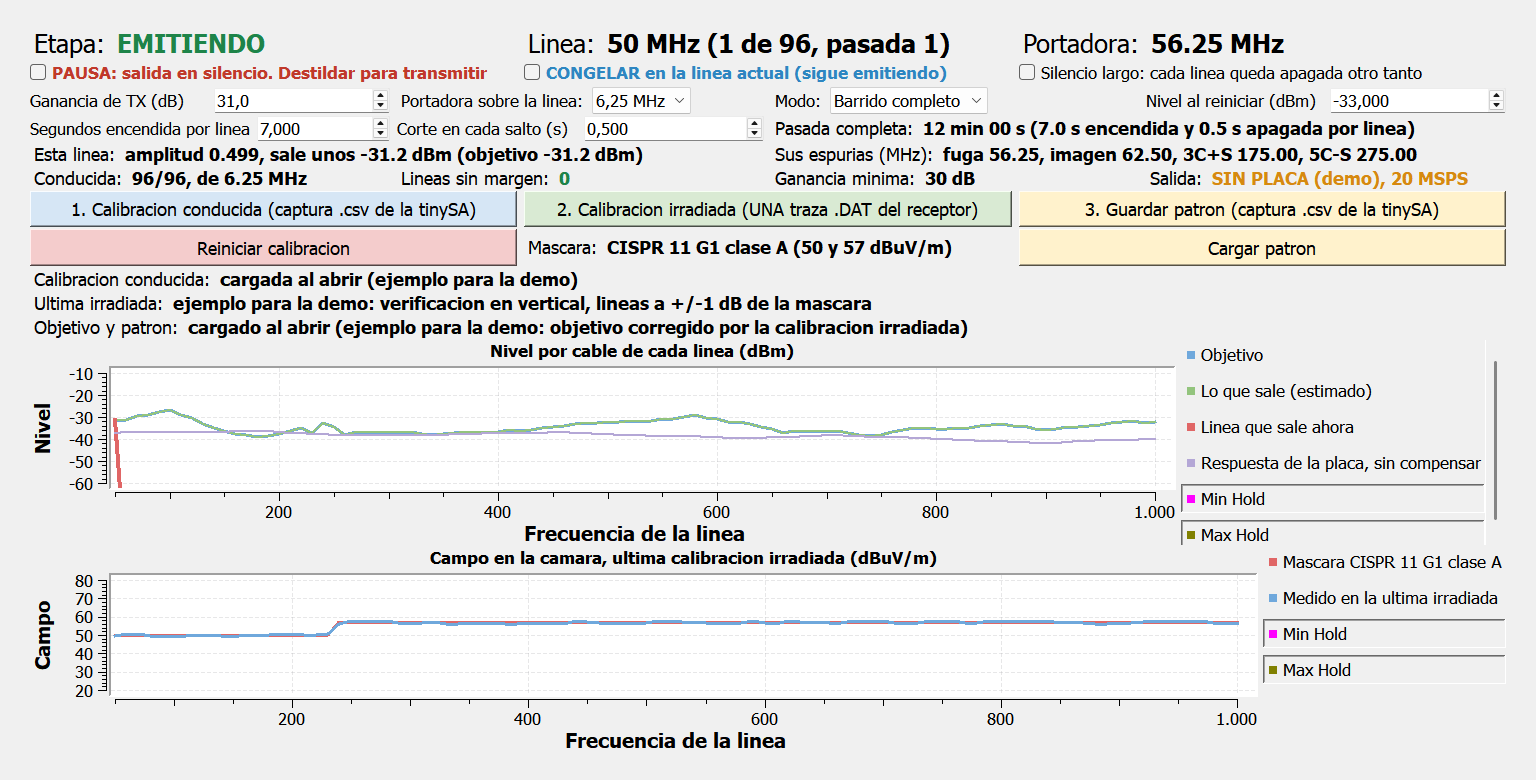
\includegraphics[width=0.92\textwidth]{fig_ventana_demo.png}
  \caption{Ventana del flujo (versión demo, con datos de ejemplo).}
\end{figure}

\begin{table}[H]
  \centering
  \small
  \begin{tabular}{@{}L{3.8cm}L{10.2cm}@{}}
    \toprule
    Control & Función \\
    \midrule
    PAUSA y CONGELAR      & Silencio, o quedarse emitiendo en la línea actual. \\
    Ganancia de TX        & Usar la ganancia mínima que muestra la ventana. \\
    Modo                  & Barrido completo o una línea fija, para orientar antenas, medir el margen sobre el piso o mirar armónicos. \\
    Nivel al reiniciar    & Objetivo plano que deja el botón Reiniciar ($-33$~dBm por defecto). \\
    Reiniciar calibración & Objetivo plano y todas las líneas con la misma amplitud. Pide confirmación y guarda una copia en respaldos. \\
    1, 2 y 3, Cargar patrón & Calibración conducida, irradiada, guardar y cargar el patrón (sección~\ref{sec:botones}). \\
    \bottomrule
  \end{tabular}
  \caption{Controles principales.}
\end{table}

\begin{itemize}
  \item Al abrir, el programa carga solo el objetivo, la calibración y la última irradiada guardados. Para cerrar: PAUSA, cerrar la ventana y esperar a que termine el proceso.
  \item La etapa cambia de color: PAUSA en rojo, CORTE en naranja, línea fija en azul y EMITIENDO en verde. Los mensajes que empiezan con NO o tienen OJO salen en rojo.
  \item Líneas sin margen: las que no llegan a su objetivo ni con amplitud 0,95. Se arreglan subiendo la ganancia.
  \item El tercer LED de la placa tiene que quedar fijo. Si titila faltan muestras por el USB y la medición no vale.
\end{itemize}

\subsection{Qué hace cada botón}\label{sec:botones}

\begin{itemize}
  \item 1. Calibración conducida: lee capturas por cable del peine tal como sale, toma el pico de cada línea (el menor entre capturas), descuenta amplitud y ganancia y calcula la amplitud que lleva cada línea a su objetivo. Dice entre cuántos dB del objetivo estaba lo leído, en verde dentro de $\pm 1$~dB. Rechaza capturas a más de 6~dB por encima o 10~dB por debajo de lo esperado.
  \item 2. Calibración irradiada: lee una sola traza del receptor, en dB$\mu$V/m, y le suma al objetivo el límite menos lo medido. Es relativa a lo cargado: otra traza hace un ajuste fino. Rechaza trazas en otra unidad, con más de una traza o ya usadas, y la traza entera si más de 10 líneas quedan a más de 15~dB del límite.
  \item 3. Guardar patrón: guarda el nivel por cable de cada línea del peine calibrado, con la ganancia, la separación y la tasa. Cargar patrón lo pone como objetivo, y la conducida reproduce la misma emisión otro día.
\end{itemize}

% ============================================================================
\section{Versiones, archivos y otro laboratorio}

\begin{itemize}
  \item Tres versiones con el mismo código: para la cámara (traza .DAT del receptor), de casa (captura .csv de un analizador con su antena, pasada a campo con $E = P + 107 + AF$) y demo (sin placa, con datos de ejemplo).
  \item Archivos de texto en la carpeta del programa, con un renglón por línea del peine: objetivo, calibración conducida, última irradiada, trazas usadas y un patrón por fecha, más la carpeta respaldos. Las versiones de casa y demo usan sus propios archivos, con el prefijo casa o demo.
  \item En otro laboratorio:
        \begin{itemize}
          \item poner el número de serie propio en el osmocom Sink,
          \item el receptor tiene que exportar un texto con el renglón y-Unit en dB$\mu$V/m y un renglón por punto con la frecuencia en Hz y el nivel, separados por punto y coma,
          \item el analizador, un .csv con la frecuencia en MHz y el nivel en dBm,
          \item el límite (CISPR~11 clase~A a 3~m) y la grilla están fijos en el bloque \texttt{limite\_lineas} y en el snippet.
        \end{itemize}
\end{itemize}

% ============================================================================
\section{Problemas frecuentes}

\begin{table}[H]
  \centering
  \small
  \begin{tabular}{@{}L{5.4cm}L{8.6cm}@{}}
    \toprule
    Síntoma & Qué hacer \\
    \midrule
    El tercer LED titila & Usar un puerto USB~3, cerrar otros programas y repetir la pasada. \\
    Error de USB o cierre inesperado & PAUSA si se puede, cerrar, desenchufar, esperar un minuto y volver a enchufar. \\
    NO se generó: en X~MHz se leyó\dots & La captura es de otra ganancia, con atenuación o al aire. Repetirla. \\
    Conducida en rojo: NO coincide & La calibración es de la otra separación. Cambiarla o calibrar de nuevo. \\
    NO se cargó: otra tasa & Calibración de una versión anterior. Reiniciar y calibrar. \\
    NO se corrigió (irradiada) & Traza en otra unidad, ya usada o que no es la del peine calibrado. Exportar otra. \\
    Líneas sin margen & Subir la ganancia a la mínima que muestra la ventana. \\
    Picos sueltos en MAX HOLD & El tono quedó encendido en un salto. Subir el corte. \\
    \bottomrule
  \end{tabular}
  \caption{Problemas frecuentes.}
\end{table}

% ============================================================================
\section{Recepción y valores preliminares}

\begin{itemize}
  \item La xA9 recibe desde 70~MHz. Sin valor publicado de entrada máxima, el criterio conservador es no superar $-15$~dBm sin atenuador.
  \item El lazo TX hacia RX por cable (EXP-18) se descartó: los armónicos del TX entran al RX y la lectura cambia de 1 a 2~dB en cada sintonía. Para RS, la medición de campo con sensores queda para el TP4.
\end{itemize}

\begin{table}[H]
  \centering
  \small
  \begin{tabular}{@{}L{4.4cm}L{9.6cm}@{}}
    \toprule
    Magnitud & Valor medido por cable con la tinySA \\
    \midrule
    Nivel de salida & Unos $-3$~dBm por línea con ganancia 65~dB y amplitud 0,25. Cae 4,5~dB de 420~MHz a 1~GHz. Comprime 0,4~dB con +3~dBm. \\
    Planitud & Sin calibrar, de $-41{,}5$ a $-36{,}8$~dBm. Calibrada, de $-34{,}6$ a $-32{,}4$~dBm contra $-33$~dBm, con desvío de 0,35~dB (40~MSPS). \\
    Fuga e imagen & Fuga de $-37$ a $-51$~dBc según la ganancia, imagen de unos $-40$~dBc. \\
    Armónicos & 3C+S de $-9$ a $-10$~dBc, 5C$-$S de $-12$ a $-17$~dBc, hasta el orden 17 a $-28$~dBc. \\
    \bottomrule
  \end{tabular}
  \caption{Valores preliminares. Los de 20 y 30~MSPS quedan por medir.}
\end{table}

% ============================================================================
\section{Referencias}

\begin{enumerate}
  \item Nuand, bladeRF 2.0 micro, documentación y libbladeRF.
  \item Analog Devices, AD9361, hoja de datos.
  \item GNU Radio 3.10 y gr-osmosdr, documentación.
  \item tinySA Ultra, manual de uso.
  \item RE-TP-001, Procedimiento de ensayo de emisiones radiadas (TP1 de este proyecto).
\end{enumerate}

\end{document}
